\documentclass[14pt]{extbook}
\usepackage{multicol, enumerate, enumitem, hyperref, color, soul, setspace, parskip, fancyhdr} %General Packages
\usepackage{amssymb, amsthm, amsmath, latexsym, units, mathtools} %Math Packages
\everymath{\displaystyle} %All math in Display Style
% Packages with additional options
\usepackage[headsep=0.5cm,headheight=12pt, left=1 in,right= 1 in,top= 1 in,bottom= 1 in]{geometry}
\usepackage[usenames,dvipsnames]{xcolor}
\usepackage{dashrule}  % Package to use the command below to create lines between items
\newcommand{\litem}[1]{\item#1\hspace*{-1cm}\rule{\textwidth}{0.4pt}}
\pagestyle{fancy}
\lhead{Progress Quiz 7}
\chead{}
\rhead{Version A}
\lfoot{4173-5738}
\cfoot{}
\rfoot{Spring 2021}
\begin{document}

\begin{enumerate}
\litem{
Solve the quadratic equation below. Then, choose the intervals that the solutions $x_1$ and $x_2$ belong to, with $x_1 \leq x_2$.\[ 20x^{2} -21 x -54 = 0 \]\begin{enumerate}[label=\Alph*.]
\item \( x_1 \in [-24.38, -23.93] \text{ and } x_2 \in [44.99, 45.07] \)
\item \( x_1 \in [-3.92, -3.51] \text{ and } x_2 \in [0.67, 1.05] \)
\item \( x_1 \in [-1.49, -1.15] \text{ and } x_2 \in [1.92, 2.37] \)
\item \( x_1 \in [-0.85, -0.48] \text{ and } x_2 \in [4.5, 4.69] \)
\item \( x_1 \in [-6.1, -5.54] \text{ and } x_2 \in [0.44, 0.53] \)

\end{enumerate} }
\litem{
Graph the equation below.\[ f(x) = -(x+4)^2 - 14 \]\begin{enumerate}[label=\Alph*.]
\begin{multicols}{2}\item 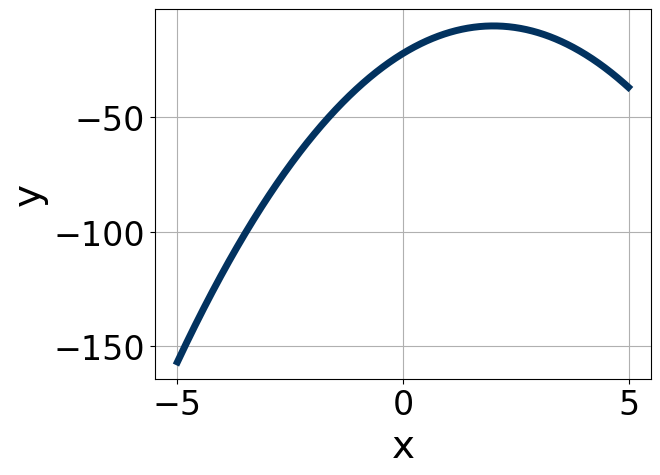
\includegraphics[width = 0.3\textwidth]{../Figures/quadraticEquationToGraphCopyAA.png}\item 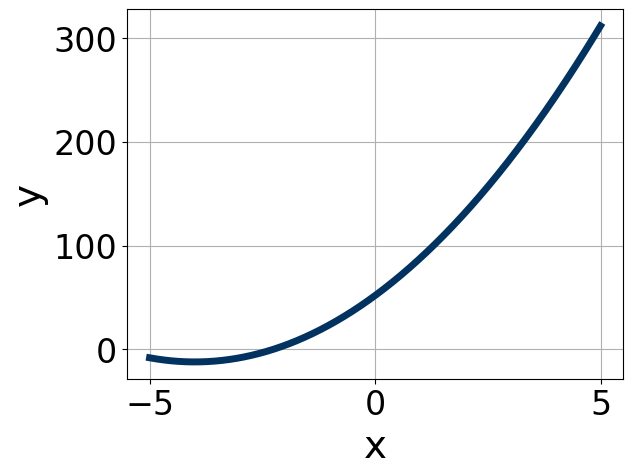
\includegraphics[width = 0.3\textwidth]{../Figures/quadraticEquationToGraphCopyBA.png}\item 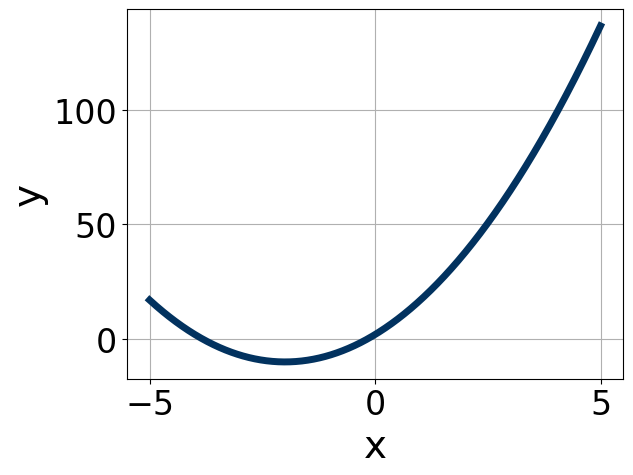
\includegraphics[width = 0.3\textwidth]{../Figures/quadraticEquationToGraphCopyCA.png}\item 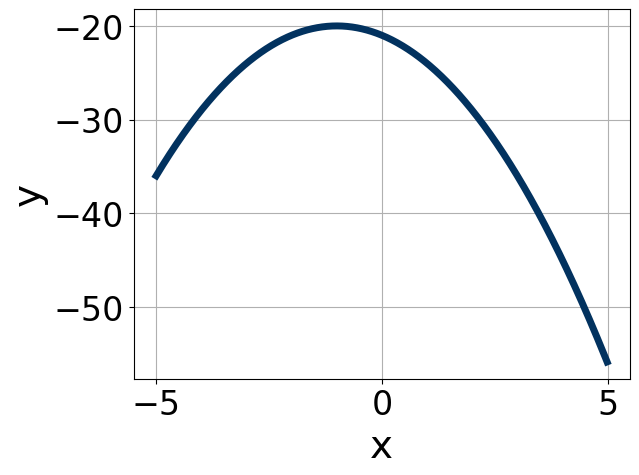
\includegraphics[width = 0.3\textwidth]{../Figures/quadraticEquationToGraphCopyDA.png}\end{multicols}\item None of the above.
\end{enumerate} }
\litem{
Solve the quadratic equation below. Then, choose the intervals that the solutions belong to, with $x_1 \leq x_2$ (if they exist).\[ 18x^{2} +10 x -4 = 0 \]\begin{enumerate}[label=\Alph*.]
\item \( x_1 \in [-1.14, -0.42] \text{ and } x_2 \in [0.05, 0.39] \)
\item \( x_1 \in [-0.72, -0.25] \text{ and } x_2 \in [0.79, 0.84] \)
\item \( x_1 \in [-15.15, -14.07] \text{ and } x_2 \in [4.65, 5.14] \)
\item \( x_1 \in [-20.94, -19.56] \text{ and } x_2 \in [19.41, 19.79] \)
\item \( \text{There are no Real solutions.} \)

\end{enumerate} }
\litem{
Solve the quadratic equation below. Then, choose the intervals that the solutions $x_1$ and $x_2$ belong to, with $x_1 \leq x_2$.\[ 15x^{2} +38 x + 24 = 0 \]\begin{enumerate}[label=\Alph*.]
\item \( x_1 \in [-2.88, -1.86] \text{ and } x_2 \in [-0.76, -0.52] \)
\item \( x_1 \in [-4.98, -3.33] \text{ and } x_2 \in [-0.43, -0.35] \)
\item \( x_1 \in [-1.53, -0.12] \text{ and } x_2 \in [-1.29, -0.76] \)
\item \( x_1 \in [-6.46, -5.63] \text{ and } x_2 \in [-0.31, -0.2] \)
\item \( x_1 \in [-20.18, -17.57] \text{ and } x_2 \in [-18.02, -17.78] \)

\end{enumerate} }
\litem{
Graph the equation below.\[ f(x) = -(x+1)^2 - 18 \]\begin{enumerate}[label=\Alph*.]
\begin{multicols}{2}\item 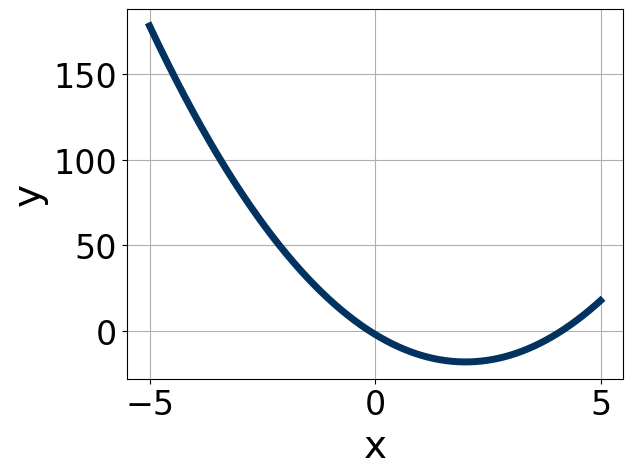
\includegraphics[width = 0.3\textwidth]{../Figures/quadraticEquationToGraphAA.png}\item 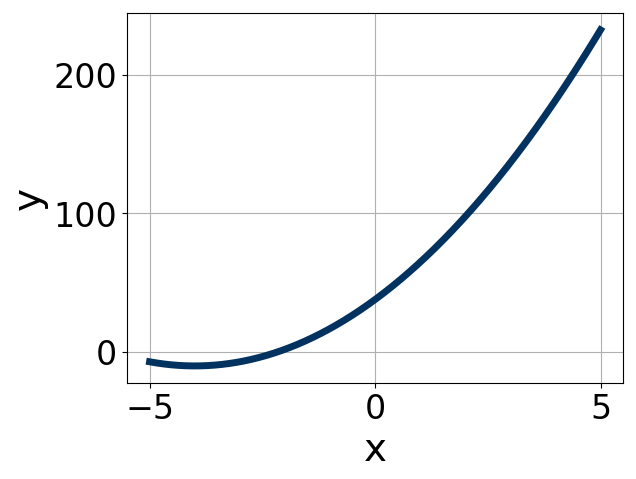
\includegraphics[width = 0.3\textwidth]{../Figures/quadraticEquationToGraphBA.png}\item 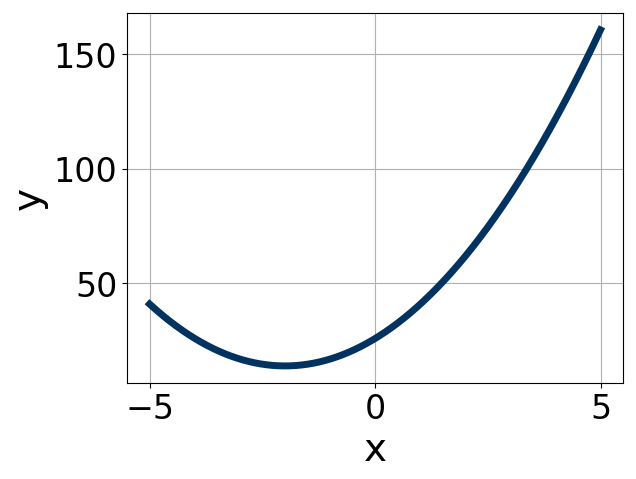
\includegraphics[width = 0.3\textwidth]{../Figures/quadraticEquationToGraphCA.png}\item 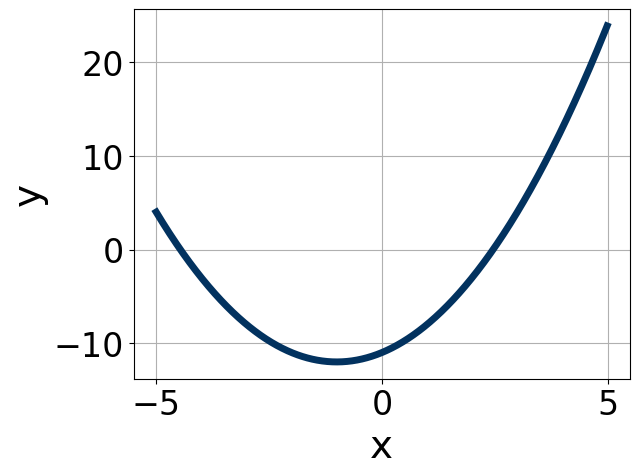
\includegraphics[width = 0.3\textwidth]{../Figures/quadraticEquationToGraphDA.png}\end{multicols}\item None of the above.
\end{enumerate} }
\litem{
Write the equation of the graph presented below in the form $f(x)=ax^2+bx+c$, assuming  $a=1$ or $a=-1$. Then, choose the intervals that $a, b,$ and $c$ belong to.
\begin{center}
    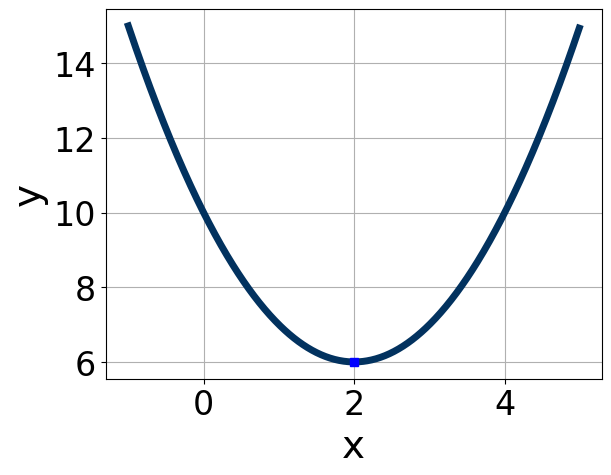
\includegraphics[width=0.5\textwidth]{../Figures/quadraticGraphToEquationA.png}
\end{center}
\begin{enumerate}[label=\Alph*.]
\item \( a \in [-1.7, -0.2], \hspace*{5mm} b \in [-5, -3], \text{ and } \hspace*{5mm} c \in [-2, 1] \)
\item \( a \in [-1.7, -0.2], \hspace*{5mm} b \in [4, 7], \text{ and } \hspace*{5mm} c \in [-2, 1] \)
\item \( a \in [0, 1.3], \hspace*{5mm} b \in [4, 7], \text{ and } \hspace*{5mm} c \in [-2, 1] \)
\item \( a \in [0, 1.3], \hspace*{5mm} b \in [4, 7], \text{ and } \hspace*{5mm} c \in [8, 9] \)
\item \( a \in [0, 1.3], \hspace*{5mm} b \in [-5, -3], \text{ and } \hspace*{5mm} c \in [8, 9] \)

\end{enumerate} }
\litem{
Factor the quadratic below. Then, choose the intervals that contain the constants in the form $(ax+b)(cx+d); b \leq d.$\[ 54x^{2} -21 x -20 \]\begin{enumerate}[label=\Alph*.]
\item \( a \in [16.1, 18.8], \hspace*{5mm} b \in [-10, -2], \hspace*{5mm} c \in [2.93, 3.34], \text{ and } \hspace*{5mm} d \in [4, 8] \)
\item \( a \in [-1.3, 1.9], \hspace*{5mm} b \in [-49, -40], \hspace*{5mm} c \in [0.97, 1.2], \text{ and } \hspace*{5mm} d \in [23, 28] \)
\item \( a \in [2.8, 4.9], \hspace*{5mm} b \in [-10, -2], \hspace*{5mm} c \in [17.42, 18.95], \text{ and } \hspace*{5mm} d \in [4, 8] \)
\item \( a \in [5.9, 8.6], \hspace*{5mm} b \in [-10, -2], \hspace*{5mm} c \in [8.18, 9.23], \text{ and } \hspace*{5mm} d \in [4, 8] \)
\item \( \text{None of the above.} \)

\end{enumerate} }
\litem{
Factor the quadratic below. Then, choose the intervals that contain the constants in the form $(ax+b)(cx+d); b \leq d.$\[ 36x^{2} +60 x + 25 \]\begin{enumerate}[label=\Alph*.]
\item \( a \in [5.31, 7.07], \hspace*{5mm} b \in [3, 9], \hspace*{5mm} c \in [4, 6.4], \text{ and } \hspace*{5mm} d \in [5, 7] \)
\item \( a \in [1.13, 2.08], \hspace*{5mm} b \in [3, 9], \hspace*{5mm} c \in [14.7, 18.3], \text{ and } \hspace*{5mm} d \in [5, 7] \)
\item \( a \in [11.66, 12.88], \hspace*{5mm} b \in [3, 9], \hspace*{5mm} c \in [1.3, 5.6], \text{ and } \hspace*{5mm} d \in [5, 7] \)
\item \( a \in [0.66, 1.73], \hspace*{5mm} b \in [28, 32], \hspace*{5mm} c \in [0.3, 2.6], \text{ and } \hspace*{5mm} d \in [30, 37] \)
\item \( \text{None of the above.} \)

\end{enumerate} }
\litem{
Write the equation of the graph presented below in the form $f(x)=ax^2+bx+c$, assuming  $a=1$ or $a=-1$. Then, choose the intervals that $a, b,$ and $c$ belong to.
\begin{center}
    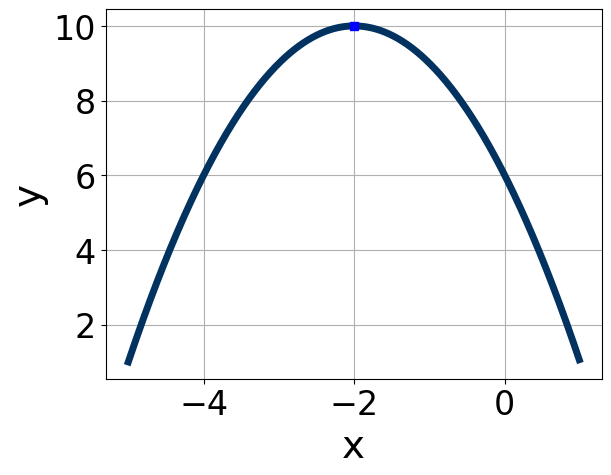
\includegraphics[width=0.5\textwidth]{../Figures/quadraticGraphToEquationCopyA.png}
\end{center}
\begin{enumerate}[label=\Alph*.]
\item \( a \in [-1.2, -0.2], \hspace*{5mm} b \in [-5, -3], \text{ and } \hspace*{5mm} c \in [-13, -8] \)
\item \( a \in [-1.2, -0.2], \hspace*{5mm} b \in [3, 6], \text{ and } \hspace*{5mm} c \in [0, 7] \)
\item \( a \in [-1.2, -0.2], \hspace*{5mm} b \in [-5, -3], \text{ and } \hspace*{5mm} c \in [0, 7] \)
\item \( a \in [-0.4, 1.3], \hspace*{5mm} b \in [3, 6], \text{ and } \hspace*{5mm} c \in [11, 14] \)
\item \( a \in [-0.4, 1.3], \hspace*{5mm} b \in [-5, -3], \text{ and } \hspace*{5mm} c \in [11, 14] \)

\end{enumerate} }
\litem{
Solve the quadratic equation below. Then, choose the intervals that the solutions belong to, with $x_1 \leq x_2$ (if they exist).\[ 20x^{2} -14 x -5 = 0 \]\begin{enumerate}[label=\Alph*.]
\item \( x_1 \in [-5.36, -5.07] \text{ and } x_2 \in [19.01, 19.78] \)
\item \( x_1 \in [-1.02, -0.57] \text{ and } x_2 \in [-0.11, 0.29] \)
\item \( x_1 \in [-0.58, -0.24] \text{ and } x_2 \in [0.69, 1.56] \)
\item \( x_1 \in [-24.99, -23.83] \text{ and } x_2 \in [24.66, 25.37] \)
\item \( \text{There are no Real solutions.} \)

\end{enumerate} }
\end{enumerate}

\end{document}